\section{آنالیز ویژگی‌های شبکه}
در ادامه فرض‌ می‌کنیم که فیلد
$sw$
در همه‌ی توصیف‌های نت‌کت پویا وجود دارد.
همچنین برای ساده‌تر شدن توصیف‌ها از اصل زیر استفاده می‌کنیم:
\begin{equation*}
    x \rat y \triangleq sw = x \cdot sw \la y
\end{equation*}

\subsection{لیست‌ سیاه}
ویژگی لیست‌ سیاه، یک لیست‌ سیاه
\lf{Blacklist}
از مکان‌هایی در شبکه وجود دارد که نباید در شبکه به آن‌ها دسترسی وجود داشته باشد
\cite{network-abstractions}
\begin{figure}
    \centering
    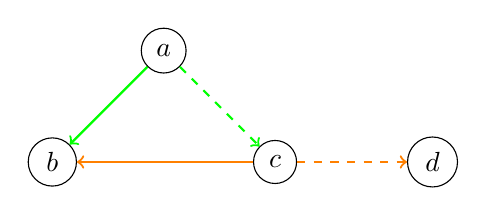
\begin{tikzpicture}[
            node distance={20mm},
            main/.style = {draw, circle},
            s/.style = {->,thick},
            d/.style = {->,thick,dashed} ]
        \node[main] (b) {$b$};
        \node[main] (a) [above right of=b] {$a$};
        \node[main] (c) [below right of=a] {$c$};
        \node[main] (d) [right of=c] {$d$};
        \draw[thick,green,->] (a) -- (b);
        \draw[thick,green,->,dashed] (a) -- (c);
        \draw[thick,orange,->] (c) -- (b);
        \draw[thick,orange,->,dashed] (c) -- (d);
    \end{tikzpicture}
    \caption{ }
    \label{fig:blacklist}
\end{figure}
به عنوان مثال شبکه‌ی رسم شده در شکل
\ref{fig:blacklist}
را در نظر بگیرید.
در این شبکه سوییچ
$d$
در لیست‌ سیاه قرار دارد، بنابراین در هیچ لحظه نباید از
$a$
که ورودی شبکه است در دسترس باشد.
در شبکه‌ی بالا ابتدا مسیر‌هایی که با خط پررنگ مشخص شده‌اند وجود دارند.
در ادامه هر یک از مسیرها با مسیر‌های خط‌چین جایگزین می‌شوند.
فرض کنید به روز رسانی این مسیر‌ها توسط دو پردازه هم‌روند انجام می‌شود.
واضح است که اگر هر دوی این به‌روز رسانی‌ها انجام شوند دسترسی به سوییچی که در لیست سیاه قرار دارد ممکن می‌شود.
اکنون فرض کنید که از عبارات زیر برای توصیف این شبکه در نت‌کت پویا استفاده کنیم:
\begin{equation*}
    \begin{aligned}[c]
        P   & = p!1                             \\
        Q   & = q!1                             \\
        N   & = F \oplus p?1;N_p \oplus q?1;N_q \\
        N_p & = F_p \oplus q?1;F_{pq}           \\
        N_q & = F_q \oplus p?1;F_{pq}           \\
        F   & = ab \oplus cb                    \\
    \end{aligned}
    \qquad\qquad
    \begin{aligned}[c]
        F_p         & = a c \oplus cb \oplus ab \\
        F_q         & = ab \oplus cd            \\
        F_{pq}      & = ac \oplus cd \oplus ad  \\
        SDN         & = \delta_{\mathcal{L}} (N
        \parallel P \parallel Q)                \\
        \mathcal{L} & = \s{p!1,p?1,q?1,q?1}     \\
    \end{aligned}
\end{equation*}
در توصیف بالا امکان اجرای هر دو به روز رسانی وجود دارد.
اکنون از مدل علی این توصیف استفاده می‌کنیم تا علت خطا را در آن پیدا کنیم.
برای توصیف مدل علی این شبکه لازم است تا ابتدا ویژگی را در قالب تابع متغیر
$PV$
توصیف کنیم.
برای این مثال تابع را به صورت زیر تعریف می‌کنیم:
\begin{align*}
    \f{PV} & = \exists c \in \mc{F}(ES(\vec v)). \exists e \in c. l(e) = ad
\end{align*}
تابع بالا رفتار نا ایمن را حالتی تعریف می‌کند که در آن امکان ارسال بسته از
$a$
به
$d$
وجود داشته باشد.

\begin{figure}
    \begin{tikzpicture}[scale=0.8]
        \crd{0}{0}{$\emptyset$}
        \crd[left]{-2}{1}{$\s{p_1}$}
        \crd[left]{-2}{2}{$\s{p_1,q_1}$}
        \crd[left]{-2}{3}{$\s{p_1,q_1,ad_1}$}
        \crd[right]{2}{1}{$\s{q_2}$}
        \crd[right]{2}{2}{$\s{p_2,q_2}$}
        \crd[right]{2}{3}{$\s{p_2,q_2,ad_2}$}
        \draw [ultra thick] (-2,1) -- (-2,2);
        \draw [ultra thick] (-2,2) -- (-2,3);
        \draw [ultra thick] (0,0) -- (2,1);
        \draw [ultra thick] (0,0) -- (-2,1);
        \draw [ultra thick] (2,1) -- (2,2);
        \draw [ultra thick] (2,1) -- (2,3);
    \end{tikzpicture}
    \caption{}
    \label{fig:blacklist:es}
\end{figure}

شکل
\ref{fig:blacklist:es}
قسمتی از نمودار ساختمان رویداد این شبکه را نشان می‌دهد که در آن تمام حالت‌هایی که
$ad$
قابل دسترس است وجود دارد.
با استفاده از مدل علی در این مثال می‌توانیم
$C(p_1,q_1) = \F$
را به عنوان یک علت برای نقض ویژگی لیست سیاه بیان معرفی کنیم در صورتی که از
$(C(p_2,q_2),\T,\T)$
به عنوان شاهد استفاده کنیم.
